\section{Chameleon Gravity}
\label{sec_cham}
We now describe \fR\ gravities exhibiting the chameleon mechanism in more detail. As stated, this mechanism uses the large mass of the chameleon field in high density regions and chameleon gravity can satisfy tests of the equivalence principle in Solar System. The action of a chameleon scalar field $\chi$ in the Einstein frame is given by the action \eqref{eq:S_ein_fr}. Varying the action with respect to the field $\chi$ one can obtain the equation of motion
\eq{
	\label{eom:cham}
	\Box\chi=V_{,\chi}-\sum_i\frac{\beta_i}{\Mpl}e^{4\beta_i\chi/\Mpl}g^\uv_{(i)}T^{(i)}_\uv,
}
where $T^{(i)}_\uv$ is the stress-energy tensor for the $i$-th matter component. For a perfect isotropic fluid the equation of motion is
\eq{
	\Box\chi=V_{,\chi}+\sum_i(1-3w_i)\frac{\beta_i}{\Mpl}\rho_i e^{(1-3w_i)\beta_i\chi/\Mpl}.
}
This equation could be read as
\eq{
	\Box\chi=V_{\eff,\chi}\left(\chi\right),
}
where the effective potential $V_{\eff}$ is defined by
\eq{
	V_{\eff}\left(\chi\right)\equiv V(\chi)+\sum_i\rho_i e^{(1-3w_i)\beta_i\chi/\Mpl}.
}
If the couplings $\beta_i$ are the same for each matter component with the same $w$ (we can omit the radiation in the sum) and the overall density is $\rho=\sum_i\rho_i$, then the effective potential reads
\eq{
	V_{\eff}\left(\chi\right)\equiv V(\chi)+\rho e^{(1-3w)\beta\chi/\Mpl}.
}
For the quasi-static and weak $(\beta\chi/\Mpl\ll1)$ field in a weak gravity background (the Minkowski background) with non--relativistic matter, the equation further simplifies as
\eq{
	\label{eq:cham}
	\Delta \chi=\frac{\beta}{\Mpl}\rho+V_{,\chi},
}
which looks like the normal Poisson equation but with an extra non--linear term.
\subsection{Chameleon Force}
The interaction of the chameleon field with matter is described by the conformal coupling \eqref{eins_trans}. Free matter fields $\psi_m^{(i)}$ follow geodesics of the Jordan frame metric. In the Einstein frame they follow modified trajectories affected by the chameleon field \parencite{Waterhouse:2006wv}
\eq{
\frac{\dd^2x^\mu}{\dd\tau^2}+\Gamma^\mu_{\alpha\beta}\dddd{x^\alpha}{\tau}\dddd{x^\beta}{\tau}=-\frac{\beta_i}{\Mpl}\left(2\chi_{,\alpha}\dddd{x^\alpha}{\tau}\dddd{x^\mu}{\tau}+g^{\beta\mu}\chi_{,\beta}\right).
}
Note that the chameleon force violates the weak Equivalence Principle only if there exist two matter species with differing values of $\beta_i$. In the non--relativistic limit, a test particle of mass $m$ of species $i$ in a static chameleon field $\chi$ is moving under a force $\mb{F}_\chi$ given by
\eq{
\label{cham_force}
\frac{\mb{F}_\chi}{m}=-\frac{\beta_i}{\Mpl}\mb{\nabla}\chi
}
\subsection{Chameleon mechanism}
As discussed previously, we need some sort of a screening mechanism to avoid Solar System tests of GR. It means as seen from \eqref{cham_force} that the chameleon potential needs to approach some constant value in dense regions or at least have a marginally suppressed amplitude.

Suppose we have a background solution $\chi_0$ which minimizes the effective potential with $\rho=\rho_0$. For small fluctuations $\chi=\chi_0+\delta\chi$ and $\rho=\rho_0+\delta\rho$ we can linearized \eqref{eq:cham} to obtain
\eq{
\label{eq:cham_lin}
\Delta \delta\chi=\frac{\beta}{\Mpl}\delta\rho+m^2_0\delta\chi,
}
where
\eq{
m^2_0\equiv V_{,\chi\chi}(\chi_0).
}
Except for the screening term the equation \eqref{eq:cham_lin} has the same behavior as the Poisson equation for the Newtonian potential $\Phi_G$. For a spherically symmetric density profile this gives solution
\eq{
\chi=\chi_0+2\beta\Mpl\Phi_G\left(r\right)e^{-m_0 r}.
}
As the objects in the background become more massive (larger and/or denser) the Newtonian potential grows larger (in magnitude) and so the deviation of $\chi$ from background solution $\chi_0$. At some point this deviation is no longer small and the potential term in \eqref{eq:cham} cannot be treated perturbatively. It starts canceling the first source term and eventually the field $\chi$ posses a new value which minimizes the effective potential inside an object.

This is the essence of the chameleon mechanism. Let us derive the mechanism in a more proper and exact way.
\subsection{Chameleon Profile}
\label{cham_prof}
To obtain the chameleon behavior described above we need to choose a chameleon potential $V(\chi)$ with the right properties. To have a screening mechanism in \eqref{eq:cham} we need $V_{,\chi}<0$ to cancel the source term and $V_{,\chi\chi}>0$ to have a real mass of the field and stable behavior of perturbations.

We wish to find a solution for spherically symmetric matter distributions of a single species of pressureless matter such that
\begin{equation*}
\rho(r)=
\begin{cases}
\rho_c & r<R_s \\
\rho_0 & r>R_s,
\end{cases}
\end{equation*}
where $\rho_c>\rho_0$. Further we define $\chi_c$ and $\chi_0$ with their masses $m_c$ and $m_0$ (the masses of small fluctuations about $\chi_c$ and $\chi_0$) such as
\begin{align*}
V_{\eff,\chi}\left(\chi_c\right)_{|\rho=\rho_c}&\equiv0	&	m^2_c&\equiv V_{\eff,\chi\chi}\left(\chi_c\right) \\
V_{\eff,\chi}\left(\chi_0\right)_{|\rho=\rho_0}&\equiv0	&	m^2_0&\equiv V_{\eff,\chi\chi}\left(\chi_0\right).
\end{align*}
In the background with low density, the curvature of the potential is much shallower, corresponding to a light scalar that mediates a long range force. Inside the object of high density, the scalar acquires a large mass, and the force shuts off.

In spherical coordinates assuming spherical symmetry, equation \eqref{eq:cham} becomes
\eq{
\label{eq_cham_r}
\frac{\dd^2\chi}{\dd r^2}+\frac{2}{r}\dddd{\chi}{r}=\frac{1}{r}\frac{\dd^2\left(r\chi\right)}{\dd r^2}=V_{,\chi}\left(\chi(r)\right)+\frac{\beta}{\Mpl}\rho(r).
}
We must impose two boundary conditions which are
\begin{align*}
\dddd{\chi}{r}(r=0)&=0 \\
\chi(r\rightarrow\infty)&=\chi_0.
\end{align*}
The first one corresponds to a non-singularity of the solution at the origin while the later one ensures that the chameleon force vanishes at the infinity (as $\dd\chi/\dd r\rightarrow0$).

The equation \eqref{eq_cham_r} drives the field $\chi$ toward the $\chi_0$ outside the object and toward $\chi_c$ inside the object. In order to solve \eqref{eq_cham_r} we must do several approximations. Outside the object we assume that the field sits near the extreme $\chi_0$ and we can linearized our equation
\eq{
\frac{1}{r}\frac{\dd^2\left(r\chi\right)}{\dd r^2}=m^2_0(\chi-\chi_0),
}
with the decaying solution
\eq{
\chi(r)=-\frac{\beta}{4\pi\Mpl}\frac{\tilde{M}}{r}e^{-m_0 r}+\chi_0.
}
Note that the integration constant $\tilde{M}$ is not generally the mass of the object $M_c$ as in the case of the Newtonian potential because it is determined by the field inside the object which has different behavior than the Newtonian potential. As we will see later, for small Newtonian potentials (in magnitude) this effective mass $\tilde{M}\approx M_c$ but as the potential grows larger part of the object`s mass is screened away $\tilde{M}< M_c$.

Inside the object we use one of the two approximations based on the initial value of $\chi_i\equiv\chi(0)$ -- either $\chi_i\approx\chi_c$ or $\chi_i\gg\chi_c$ .
\subsubsection{Thin-shell regime}
In the \textit{thin-shell} regime the field initially sits very close the minimum $\chi_c$, i.e. we require
\eq{
(\chi_i-\chi_c)/\chi_c\ll1.
}
The field is frozen near this value until the friction term is sufficiently small to allow the field to roll. This ``moment'' is denoted by $R_{roll}$. As soon as $\chi$ is displaced significantly from $\chi_c$ we may neglect the potential term in \eqref{eq_cham_r}. This gives us the solution
\eq{
\chi(r)=
\begin{cases}
\chi_c & 0<r<R_{roll} \\
\frac{\beta}{6\Mpl}\rho_cr^2+\frac{A}{r}+D & R_{roll}<r<R_s.
\end{cases}
}
We have boundary conditions coming from the requirement on matching $\chi$ and  $\dd\chi/\dd r$ at $R_{roll}$, namely: $\chi=\chi_c$ and $\dd\chi/\dd r=0$ at $r=r_{roll}$. This fixes our constants and the solution is
\eq{
\label{eq_thin}
\chi(r)=
\begin{cases}
\chi_c & 0<r<R_{roll} \\
\frac{\beta\rho_c}{3\Mpl}\left(\frac{r^2}{2}+\frac{R^3_{roll}}{r}\right)-\frac{\beta\rho_cR^2_{roll}}{2\Mpl}+\chi_c & R_{roll}<r<R_s.
\end{cases}
}
The approximation of separating the solution into the two regions only makes sense if $(R_s-R_{roll})/R_s\ll1$. Otherwise there is no clear separation between the two regions, and one needs a solution valid over the entire range $0<r<R_s$. In \autoref{sec:num_cham} we solve equation \eqref{eq_cham_r} numerically and we will check these approximations against numerical solutions.

With approximation $(R_s-R_{roll})/R_s\ll1$ we can determines the effective mass of the object $\tilde{M}$ from the requirement $\chi(R_s^-)=\chi(R_s^+)$ and $\dd\chi/\dd r(R_s^-)=\dd\chi/\dd r(R_s^+)$.
\eq{
\tilde{M}=\frac{3\Delta R_s}{R_s}M_c,
}
where
\eq{
\frac{\Delta R_s}{R_s}\equiv\frac{\chi_0-\chi_c}{6\beta\Mpl|\Phi_G(R_s)|}\approx\frac{R_s-R_{roll}}{R_s}\ll1.
}
This qualitative derivation of the thin-shell regime is using too much strong assumptions and can be done more precisely without ignoring some of the terms but then it is harder to see the principle of the thin-shell effect. For more details see e.g. \textcite{Tamaki:2008mf,2007PhRvD..75f3501M,Waterhouse:2006wv}.
\subsubsection{Thick-shell regime}
In the \textit{thick-shell} regime the field is initially sufficiently displaced from the minimum -- $\chi_i\gg\chi_c$ that it begins to roll almost immediately (no friction term). Hence the interior solution is most easily obtained by taking the $R_{roll}=0$ in \eqref{eq_thin} and replacing $\chi_c$ by $\chi_i$
\eq{
\label{eq_thick}
\chi(r)=\frac{\beta\rho_cr^2}{6\Mpl}+\chi_i\ \ \ 0<r<R_s.
}
By matching the interior and exterior solutions, we obtain
\eq{
\begin{split}
\chi_i &=\chi_0-3\beta\Mpl\Phi_G(R_s)\\
\tilde{M} &=M_c,
\end{split}
}
which is the linear regime with no screening. From the definition of $\Delta R_s/R_s$ we also obtain
\eq{
\frac{\Delta R_s}{R_s}\equiv\frac{\chi_0-\chi_c}{6\beta\Mpl|\Phi_G(R_s)|}>1.
}
\subsubsection{Thin-shell suppression factor}
The chameleon force outside the object (where experiments take place) comparing to the Newtonian force is
\eq{
\begin{split}
\label{eq_cham_suppression}
\frac{F_{thick}}{F_N}&=2\beta^2 \\
\frac{F_{thin}}{F_N}&=2\beta^2\frac{3\Mpl\left(\chi_0-\chi_c\right)}{\beta\rho_cR^2_c},
\end{split}
}
where we ignore the term $m_0 r\ll1$. Therefore for the coupling $\beta$ of order unity the chameleon force is as strong as gravity unless it is screened away by the thin-shell effect.
%%%%%%%%%%%%%%%%%%%%%%%%%%%%%%
% HU-SAWICKI
%%%%%%%%%%%%%%%%%%%%%%%%%%%%%%
\subsection{Hu-Sawicki \texorpdfstring{\textit{\lowercase{f}(R)}}{fR} Model}
We wish to study a class of $f(R)$ models that accelerate cosmic expansion at late times, without the cosmological constant, while satisfying both cosmological and Solar System tests. We consider the family of Hu-Sawicki $f(R)$ models \parencite{Hu-Saw}. The action of these models is given by \eqref{eq:S_fr} and $f(R)$ has a broken power-law form
\eq{
	f(R)=-M^2\frac{c_1(R/M^2)^m}{c_2(R/M^2)^m+1}\,,
}
where the mass scale $M^2\equiv\bar\rho_0/3\Mpl^2$, $m>0$, and $c_1$ and $c_2$ are dimensionless parameters such that at high redshifts \LCDM\ cosmology is restored.

The formulation of modified gravity in this frame leads to second-order differential equations of motion \eqref{eq:fR} for $R$ and fourth-order field equations for $g_\uv$. With a conformal transformation \eqref{eins_trans} we may rewrite these equation in the Einstein frame with second-order differentials only \parencite[see, e.g.,][]{CHIBA20031}. In the Einstein frame, the Hu-Sawicki models correspond to chameleon gravity with the potential
\eq{
	V(\chi) &= \Mpl^2\Lambda-\frac{\beta\bar\rho_0}{n\Mpl}\left(2\beta\Mpl\Phiscrz\right)^{1-n}\chi^n\,, \\
    V_{,\chi}(\chi) &= -\frac{\beta}{\Mpl}\bar\rho_0\left(\frac{2\beta\Mpl\Phiscrz}{\chi}\right)^{1-n}\,,
}
where $\beta=\sqrt{1/6}$ and the power-law exponent $n$ and screening potential $\Phiscrz$ are now the free parameters of the theory. The screening potential has the following relation to the present scalaron value in $f(R)$-gravity:
\eq{
    \Phiscrz=\frac{3}{2}\ln{(1+f_{R0})}\approx\frac{3}{2}f_{R0}.
}
The chameleon obeys the equation of motion \eqref{eom:cham} which reduces for our study case (non--relativistic pressureless matter) to
\eq{
\label{eq:cham_husa}
	\Delta \chi = \frac{\beta}{\Mpl}\rho - \frac{\beta}{\Mpl}\bar\rho_0\left(\frac{2\beta\Mpl\Phiscrz}{\chi}\right)^{1-n}
}
We rescale the equations to units in which we can clearly see the role of the screening potential $\Phiscr$ and its relation to the gravitational potential $\Phi_G$. We start by defining a few special values of the chameleon potential -- the current background value
\eq{
	\chi_0\equiv2\beta\Mpl\Phiscrz\,,
}
the background value at a given time (for a matter dominated universe)
\eq{
	\chi_a(a)\equiv \chi_0 a^{3/(1-n)}
}
and the value of the screening potential at a given time
\eq{
	\Phiscra\equiv\Phiscrz a^{\frac{5-2n}{1-n}}\,.
}
With these definitions we rewrite equation \eqref{eq:cham} as
\eq{
\label{eq:cham_u}
	\Delta\left(\chi/\chi_a\right)= C_\chi(a)\left[1+\delta-\left(\frac{\chi_a}{\chi}\right)^{1-n}\right]\,,
}
where the pre-factor $C_\chi(a)$ is defined by
\eq{
	C_\chi(a)\equiv\frac{3H_0^2\Omega_m}{2\Phiscrz}a^{-3\frac{2-n}{1-n}}=\left(a\mu\Phiscra\right)^{-1}\,.
}
\subsubsection{Linear prediction}
Equation \eqref{eq:cham_u} is similar to the Poisson equation for the gravitational potential and gives meaning to the screening potential $\Phiscra$. If we assume $\chi\approx\chi_a$, then
\eq{
	\label{eq:chi__scr_mean}
	\Delta\left(\chi/\chi_a\right) \approx \left(\mu\Phiscra\right)^{-1}\frac{\delta}{a} = \Delta\left(\Phi_G/\Phiscra\right)
}
and we can write down a linear solution as
\eq{
\label{eq:chi_lin_x}
	\chi(\mb x, a) = \chi_a(a)\left(1 + \frac{\Phi_G(\mb x, a)}{\Phiscra(a)} \right)\,.
}
Here we can clearly see the role of the (time dependent) screening potential $\Phiscra$ -- as long as $|\Phi_G| < \Phiscra$ we have a valid solution but once the gravitational potential is large enough (in its negative values) the linear solution breaks down, as the chameleon field would become negative.

We may derive a more accurate solution in Fourier space. If the chameleon field sits near its background value, i.e. $\chi=\chi_a\left(1 + \delta\tilde\chi \right)$, where $\delta\tilde\chi \ll 1$, we can rewrite \eqref{eq:cham_u} as
\eq{
	\Delta\delta\tilde\chi=\frac{m^2}{1-n}\delta + m^2\delta\tilde\chi\,,
}
where the mass of the chameleon field is
\eq{
    \label{eq:chi_m}
	m^2(a)\equiv\frac{1-n}{a\mu\Phiscra}\,.
}
This equation has a solution in $k-$space of the form
\eq
{
\label{eq:chi_lin_k}
	\hat{\chi}(k)=-\frac{\chi_a}{1-n}\frac{m^2}{m^2+k^2}\hat{\delta}(k) = -\frac{\beta\bar\rho}{\Mpl}\frac{\hat{\delta}(k)}{k^2+m^2}\,.
}

The other regime, which can be solved approximately, is the screened regime inside massive objects. When the solution \eqref{eq:chi_lin_x} breaks down, and if $\delta(x)$ is approximately constant, the solution of equation \eqref{eq:cham_u} is
\eq{
	\chi=\frac{\chi_a}{\left(1+\delta\right)^{1/(1-n)}}\,.
	\label{eq:chi_bulk}
}
Because $\chi_a$ is constant in space the chameleon force \eqref{cham_force} vanishes in this screened regime.

In \autoref{fig:chi_evol} we show the evolution of background parameters of the chameleon field -- Compton wavelength $\lambda_c=m^{-1}$, background value of the chameleon field $\chi_a$ and the screening potential $\Phiscra$ -- for different values of the power-law exponent $n$ and the screening potential $\Phiscrz$.

\begin{figure}[hbt]
\centering
	\begin{subfigure}{1.0\textwidth}
        \includegraphicscustomlegend{modif_grav/chi_evol}
	\end{subfigure}
	\begin{subfigure}{1.0\textwidth}
		\includegraphicscustom{modif_grav/chi_evol}
	\end{subfigure}
    \caption{Evolution of background parameters of the chameleon field. From top to bottom: Compton wavelength $\lambda_c$, chameleon field $\chi_a$ and screening potential $\Phiscra$.}
    \label{fig:chi_evol}
\end{figure}

The background value of the Compton wavelength informs us about the global behavior of the chameleon field whereas the screening potential describes its behavior locally. At high redshifts, the chameleon's Compton wavelength is too short to have any effects -- on large scales, due to its low background value, and on small scales due to a low value of the screening potential. At lower redshifts the chameleon field starts to affect matter, initially only on small scales but with the passage of time also on large scales. We thus expect the strongest effects to be on small scales.
\subsection{Numerical solutions}
\label{sec:num_cham}
In this section we will show results of results of numerical solutions of chameleon profile. We will solve the equations for Hu-Sawicki \fR\ model, \eqref{eq:cham_husa}. In this section we will focus only on systems with spherical symmetry \eqref{eq_cham_r}, i.e. we will solve the the following equation
\eq{
	\label{eq:cham_husa_r}
	\frac{\dd^2\chi}{\dd r^2}+\frac{2}{r}\dddd{\chi}{r} = \frac{\beta}{\Mpl}\rho - \frac{\beta}{\Mpl}\bar\rho_0\left(\frac{\chi_0}{\chi}\right)^{1-n}
}
Our algorithm for finding solutions to \eqref{eq:cham_husa_r} uses the shooting method \parencite{10.5555/42249} and is based on the original algorithm of \textcite{mastersthesis_vrastil}. We further improved the code applicability, readability and its parametrization. The code is publicly available at \code{\url{https://github.com/vrastil/chi_r_solver}}.

\subsubsection{Stars}
We will first consider a case where some approximate solutions exists -- a compact spherical object of constant density $\rho_c$ surrounded by the background of density $\rho_0$ as discuss in \autoref{cham_prof}. We expect that for low-mass objects the chameleon field will track the Newtonian potential while for massive objects the chameleon field will be frozen inside the sphere and outside it will be following the Newtonian behavior but with decreased amplitude.

In \autoref{fig:starlike} we show results for the chameleon profile. We used the notation $\tilde\chi\equiv(\chi-\chi_0)/2\beta\Mpl$ for better comparison with the Newtonian potential. We see that for $\Phiscr>\Phi_G$ we have an unscreened solution as expected. For lower values of $\Phiscr$ the field is frozen inside the object and have lower amplitude outside the object as expected from analytical solutions.
\begin{figure}
	\centering
	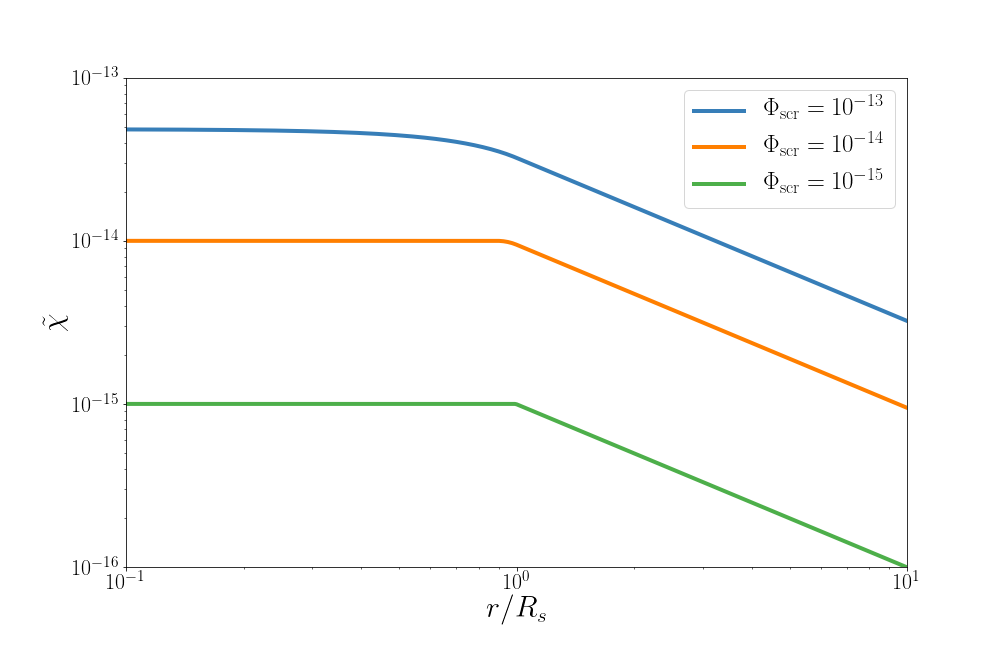
\includegraphics[width=1.0\linewidth]{{spherical_cham/starlike}.png}
	\caption{Chameleon profile for several screening potentials. The top solution is in the linear regime and is identical to the gravitational potential. The other two solutions are in the screened regime and the amplitude of the field is suppressed.}
	\label{fig:starlike}
\end{figure}

Let us focus on the regime which cannot be treated analytical, i.e. regime between thin-shell and thick-shell solutions. This regime corresponds to the situation when the linear approximation (thick-shell) breaks down inside the object, i.e. the gravitational potential cancels screening potential somewhere inside the object.We will denote $\Req$ the \textit{equivalence radius} -- radius at which the Newtonian potential equals the screening potential $|\Phi_G(\Req)|=\Phi_s$. By letting the equivalence radius posses also negative values such as $(1+|\Req|/R_s)|\Phi_G(0)|=\Phi_s$ we can clearly distinguish between the linear $(\Req<0)$ and the screening $(\Req>0)$ regime.

In \autoref{fig:starlike_forces} we show the behavior of the chameleon fifth force in this regime. We see that for the linear regime the fifth force is as strong as standard gravity (up to the factor $2\beta^2$). For $\Req\ll R_s$ the chameleon field manages to catch up the linear solution inside the object and there is no screening outside. As the $\Req$ grows the field is not able catch up the linear solution while inside the object and the force outside is screened.
\begin{figure}
	\centering
	
\includegraphics[width=1.0\linewidth]{{spherical_cham/starlike_forces}.png}
	\caption{Chameleon force relative to the standard gravitational force for several screening potentials (given through the equivalence radius). For $\Req\ll R_S$ there is no screening outside the object. As the $\Req$ grows the chameleon enters the screened regime.}
	\label{fig:starlike_forces}
\end{figure}

\subsubsection{NFW Halo}
The Navarro-Frenk-White (NFW) profile proposed by \textcite{1996ApJ...462..563N} describes the distribution of cold dark matter. The NFW profile of matter overdensity is given by
\eq{
	\label{NFW_rho}
	\delta\rho_{NFW}(r)=\frac{\rho_c}{r/r_s\left(1+r/r_s\right)^2},
}
where $\rho_c$ is the density scale and $r_s$ is the scale radius. We will also be using the dimensionless radius $x\equiv r/r_s$. Total mass of the halo is divergent (logarithmically) so we take a cut-off at the radius $r_{200}$, which is defined as the radius at which the density is 200 times the critical density. Then the mass of the halo is
\eq{
	M_{200}=\int_0^{r_{200}}4\pi r^2\rho(r)\dd r=4\pi\rho_cr_s^3\left(\ln(1+c)-\frac{c}{c+1}\right),
}
where $c\equiv r_{200}/r_s$ is the concentration of the halo. For a given mass the halo is fully characterized by the concentration.

For NFW halo the density is not constant as in the case of compact spherical objects (stars). The chameleon mass and the screened solution is therefore also not constant and one does not have analytical solutions as in the case of stars. However, for realistic halo the density varies on scales much larger than the Compton wavelength of the chameleon. In such cases we can treat the field as frozen in the same sense as in the case of stars. Therefore we expect the chameleon field to behave in a similar way as in the case of stars, i.e. to follow the Newtonian potential in the linear case and to have screened behavior for more massive halos.

In \autoref{fig:nfwlike_forces} we show the chameleon fifth force. We see that the behavior is indeed similar to stars although the field catches up much later. This is due to the fact that there is no sudden drop in density (and mass of the field) where the chameleon can start to behave as free but rather the mass is slowly dropping. This indicates that it will be much harder to detect the chameleon fifth force on scales of galaxies than for star-like objects. This is of course true only assuming the screening potential is the same on all scales.
\begin{figure}
	\centering
	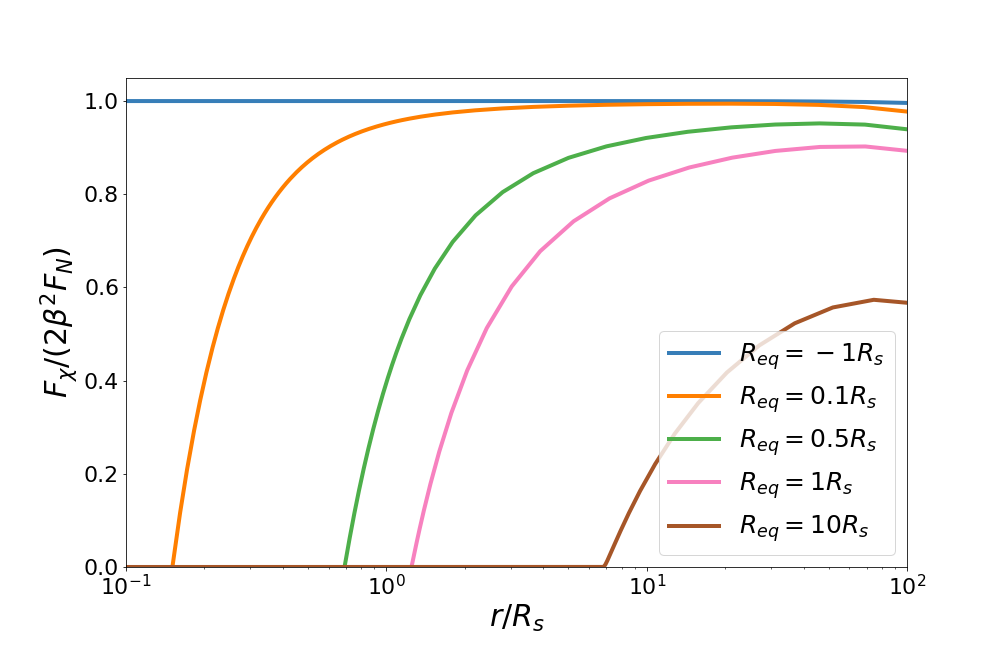
\includegraphics[width=1.0\linewidth]{{spherical_cham/nfwlike_forces}.png}
	\caption{Chameleon force relative to the standard gravitational force for several screening potentials (given through the equivalence radius). For $\Req\ll R_S$ there is no screening outside the object. As the $\Req$ grows the chameleon enters the screened regime.}
	\label{fig:nfwlike_forces}
\end{figure}

The meaning of the screening potential and its connection to the Newtonian potential in \eqref{eq:chi__scr_mean} is given by the value of the field at the background, i.e. value that minimizes right side of \eqref{eq:cham_u}. However, objects like stars or galaxy halos do not sit directly in the overall average density of the universe but rather in galaxy halo or halo of the cluster of galaxies. Therefore the value of the effective screening potential is given by the density the background object we can consider as being in infinity relative to the scale of studied object. In \autoref{fig:nfwlike_pot_eff} we show the value of this effective screening potential for a cluster of galaxies of a typical size -- $M=10^{14} M_\odot, c=4$. We see that the screening potential is greatly reduced in inner parts of the galaxy cluster halo. For this reason we do not think it much likely to observe effects of the chameleon field on scales smaller than Mpc.

\begin{figure*}
	\centering
		\begin{subfigure}{1.0\linewidth}
			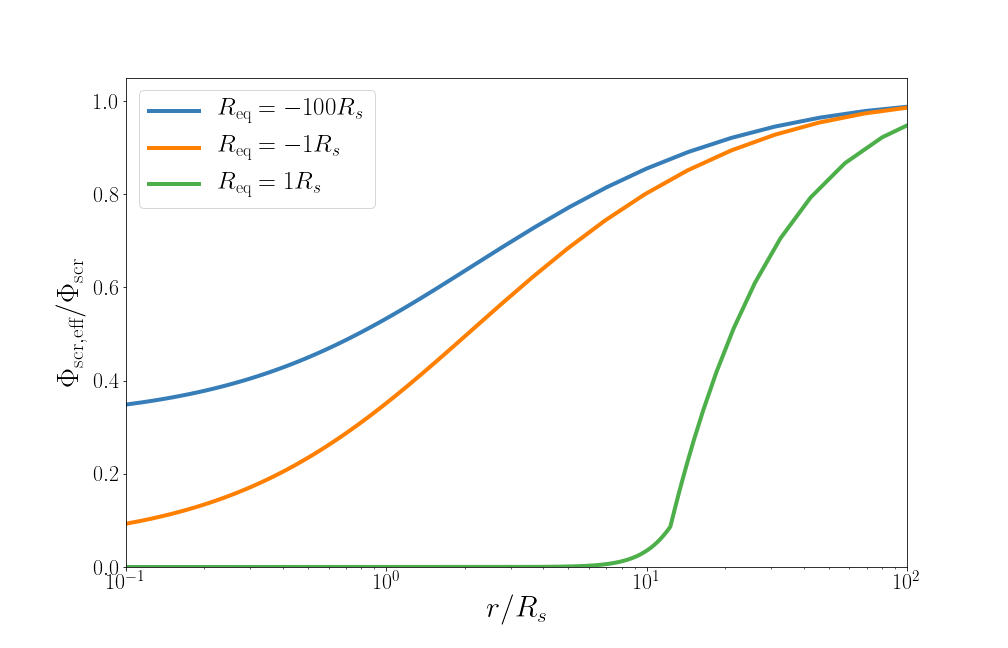
\includegraphics[width=1.0\linewidth]{{spherical_cham/nfwlike_pot_eff}.png}
		\end{subfigure}
		\begin{subfigure}{1.0\linewidth}
			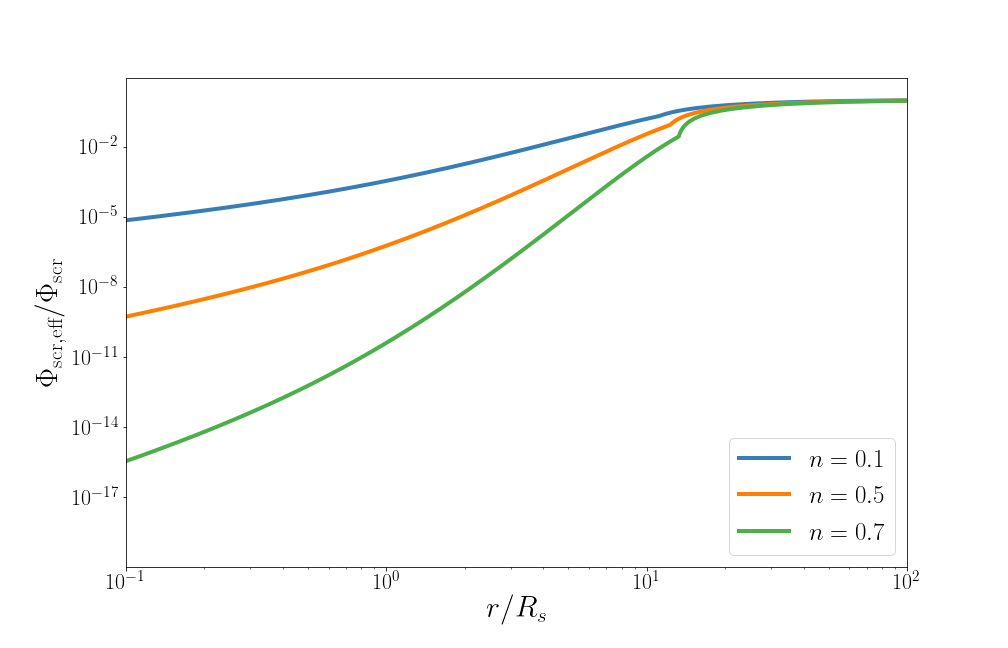
\includegraphics[width=1.0\linewidth]{{spherical_cham/nfwlike_pot_eff_n}.png}
		\end{subfigure}
		\caption{Effective screening potential relative to the screening potential for a cluster of galaxy, $M=10^{14} M_\odot, c=4$. Top Figure is shown for several screening potentials (given through the equivalence radius) while the bottom for different chameleon parameter $n$.}
		\label{fig:nfwlike_pot_eff}
\end{figure*}

As the chameleon affects only non--relativistic matter it can be detected using combination of dynamical measurements and lensing measurements. Therefore, we considered what would be difference between mass distribution of a galaxy cluster measured via lensing (true mass) and via dynamics of enclosed galaxies. In \autoref{fig:clustersYs} we plot this ratio for five real clusters (simulated as having ideal NFW profile), see their parameters in \autoref{tab:clusters}, and for four different values of the screening potential. We see that except for the case $\Phiscr=1$ one would need very precise (and nowadays unrealistic) measurements of the mass distribution. We are therefore left with only cosmological scales of tens of Mpc and larger to study the chameleon. We will study this case in \autoref{chpt:app_sims}.
\begin{table}[hbt]
	\begin{tabular}{lcc|lcc}
		\hline \hline
		Cluster & $c$ & $M$ & Cluster & $c$ & $M$ \\
		\hline
		ClG 0054-27 & $1.2$ & $0.42\cdot10^{14}$ &
		Cl 0016+1609 & $2.1$ & $1.12\cdot10^{14}$ \\
		MS 2137.3-2353 & $13$ & $2.9\cdot10^{14}$ &
		ClG 2244-02 & $4.3$ & $4.5\cdot10^{14}$ \\
		MS 0451.6-0305 & $5.5$ & $18\cdot10^{14}$ & & & \\
		\hline \hline
	\end{tabular}
	\caption{Properties of clusters simulated as perfect NFW halos: concentration $c$ and mass $M [M_\odot]$. Parameters are taken from \textcite{2007MNRAS.379..190C}}
	\label{tab:clusters}
\end{table}

\begin{figure*}[!hbt]
\begin{adjustwidth}{-1cm}{-1cm}
	\centering
		\begin{subfigure}{0.5\linewidth}
			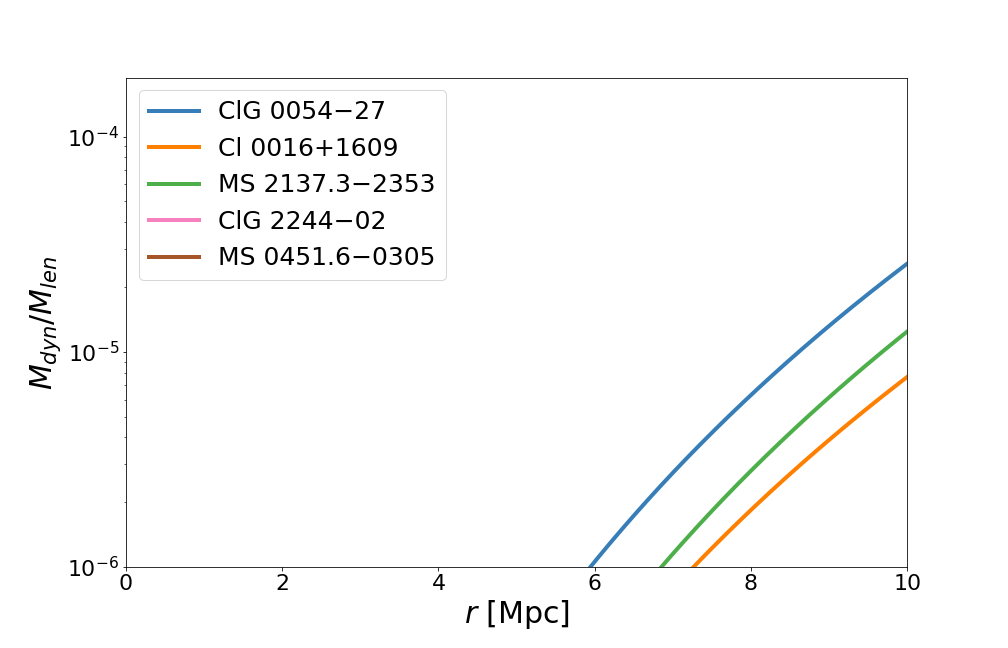
\includegraphics[width=1.0\linewidth]{{spherical_cham/clustersYs_-6}.png}
			\caption{$\Phiscr=10^{-6}$}
		\end{subfigure}%
		\begin{subfigure}{0.5\linewidth}
			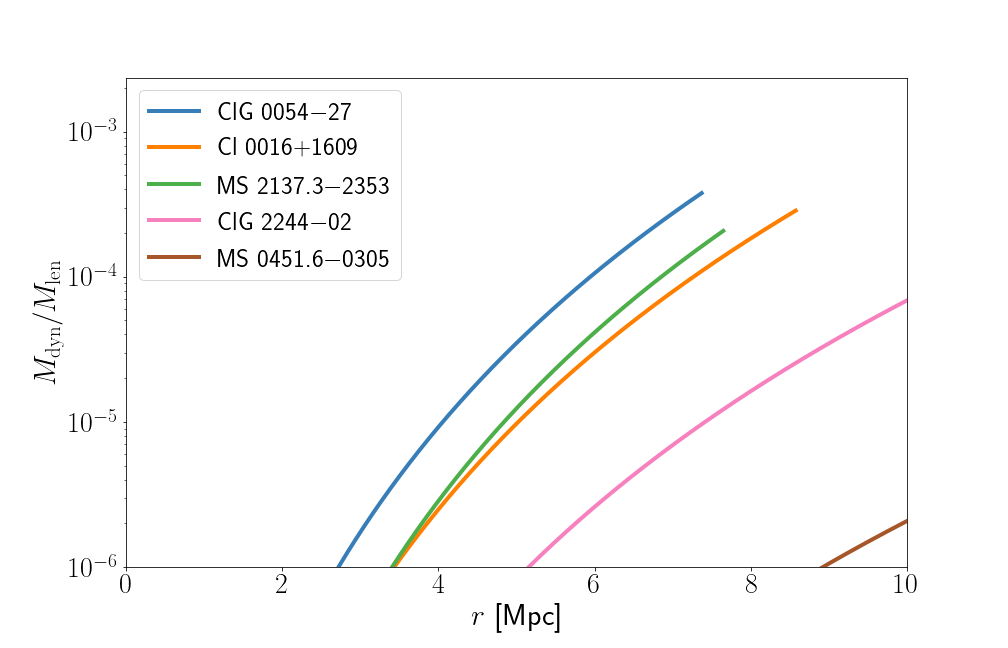
\includegraphics[width=1.0\linewidth]{{spherical_cham/clustersYs_-4}.png}
			\caption{$\Phiscr=10^{-4}$}
		\end{subfigure}
		\begin{subfigure}{0.5\linewidth}
			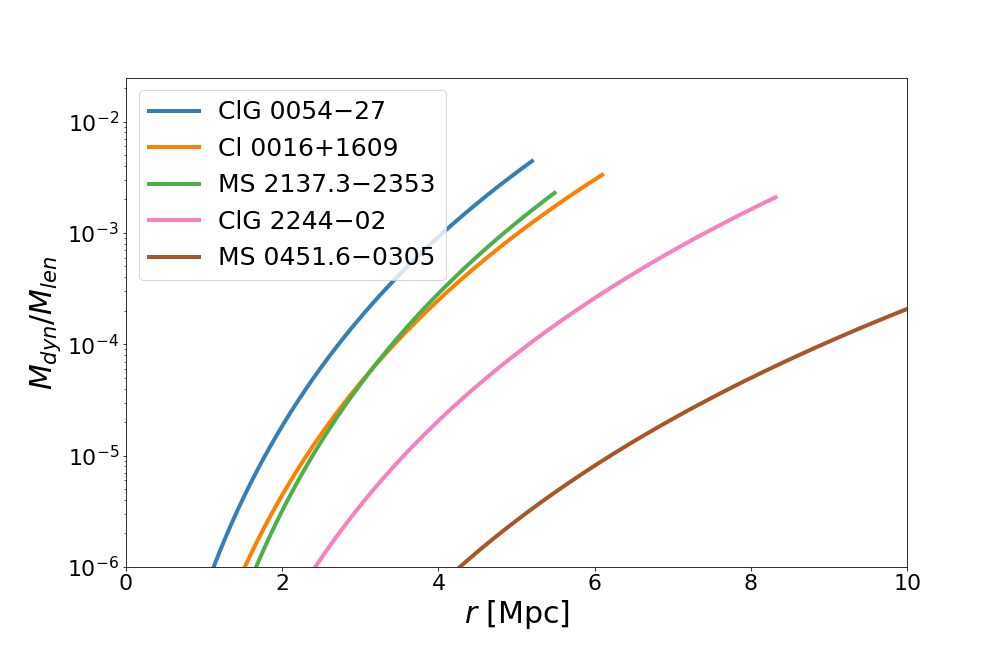
\includegraphics[width=1.0\linewidth]{{spherical_cham/clustersYs_-2}.png}
			\caption{$\Phiscr=10^{-2}$}
		\end{subfigure}%
		\begin{subfigure}{0.5\linewidth}
			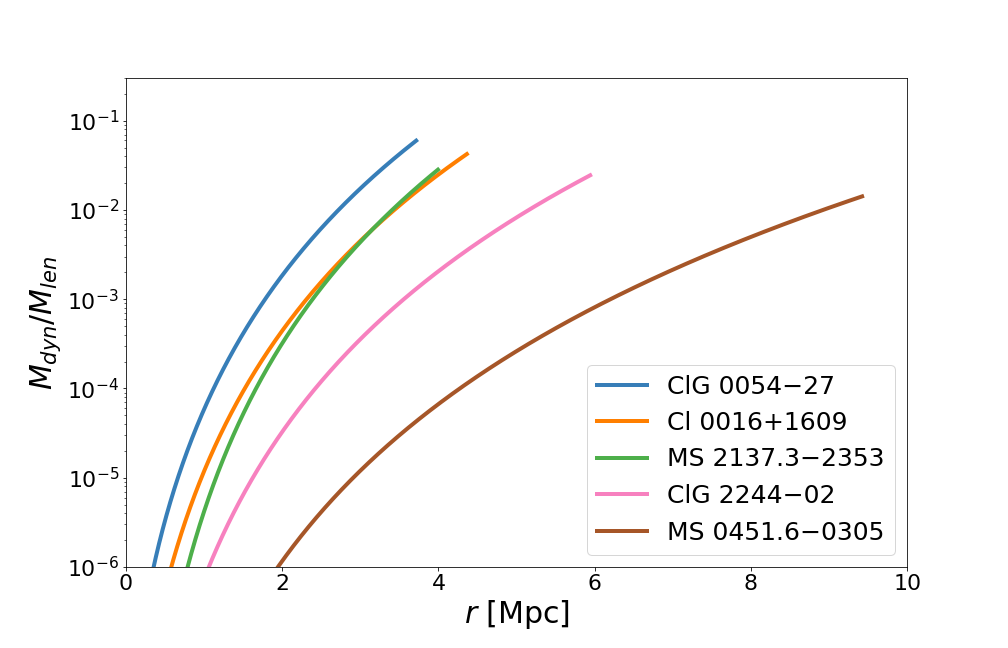
\includegraphics[width=1.0\linewidth]{{spherical_cham/clustersYs_0}.png}
			\caption{$\Phiscr=10^{0}$}
		\end{subfigure}
	\end{adjustwidth}
		\caption{Effective dynamical mass of the clusters relative to the actual (lensing) mass of the cluster. Cluster properties are shown in \autoref{tab:clusters}.}
		\label{fig:clustersYs}
\end{figure*}